\documentclass[12pt,a4paper]{article}

\clubpenalty=100000 
\widowpenalty=100000 

\usepackage{cobengesty}

\makeatletter 
\renewcommand\@biblabel[1]{} 
\makeatother

\title{INSTRUÇÕES PARA A PREPARAÇÃO E SUBMISSÃO DE TRABALHOS AO COMITÊ CIENTÍFICO DO XLIV CONGRESSO BRASILEIRO DE EDUCAÇÃO EM ENGENHARIA}


\begin{document}

\maketitle

%%%%%%%%%%%%%%%%%%%%%%%%%%%%%%%%%%%%%%%%%%%%%%%%%%%%%%%%%%%%%%%%%%%%
%OBSERVAÇÃO: O NOME DOS AUTORES SÓ DEVE CONSTAR NA VERSÃO FINAL %%%%
%Comente na primeira versão (antes da revisão)  				%%%%
%%%%%%%%%%%%%%%%%%%%%%%%%%%%%%%%%%%%%%%%%%%%%%%%%%%%%%%%%%%%%%%%%%%%

\autor{Primeiro Autor}\email{primeiro.autor@cobenge.br}
\infoautor{Instituição de Ensino, Faculdade ou Departamento}{Endereço}{CEP}{Cidade}{Estado}

\autor{Segundo Autor}\email{segundo.autor@cobenge.br}
\infoautor{Instituição de Ensino, Faculdade ou Departamento}{Endereço}{CEP}{Cidade}{Estado}

\autor{Primeiro Autor}\email{primeiro.autor@cobenge.br}
\infoautor{Instituição de Ensino, Faculdade ou Departamento}{Endereço}{CEP}{Cidade}{Estado}


\begin{abstract}
Este documento apresenta instruções para a preparação e submissão de trabalhos para o COBENGE 2016, com base em edições anteriores. O trabalho deve atender às seguintes especificações: a) digite o corpo do texto em uma única coluna; b) utilize um máximo de 16 páginas tamanho A4 (21 x 29,7 cm), cada qual com margens esquerda, direita, e inferior iguais a 2,5 cm e superior igual a 3,0 cm (não inclua molduras ou números de página); c) use a fonte Times New Roman tamanho 14 pt para o título e 12 pt para subtítulos e corpo do texto. Os tamanho mínimo de fonte para tabelas e figuras é de 10 pt; d) prepare um resumo com um máximo de 250 palavras em itálico seguido de no máximo cinco palavras-chave; e) use espaçamento simples e alinhamento justificado para os parágrafos; f) as referências devem ser listadas em ordem alfabética no final do trabalho, segundo a norma NBR 6023; g) as figuras/fotografias incluídas no trabalho devem ser de boa qualidade (300 dpi/jpg). O trabalho poderá ser preparado em português, espanhol ou inglês. Um arquivo no formato PDF deverá ser submetido eletronicamente até o dia 05 de JUNHO de 2016, através do JEMS (Journal and Event Management System) no endereço https://submissoes.sbc.org.br/. Instruções sobre como enviar trabalhos estão disponíveis na página do evento http://www.abenge.org.br/cobenge-2016/ na aba “Submissão de trabalhos” a partir do dia 04.04.2016.
\end{abstract}
%
\begin{keywords}
Primeira palavra, Segunda palavra, Terceira palavra (máximo de 5).
\end{keywords}

\section{INTRODUÇÃO}

Os Anais do COBENGE 2016 serão publicados incluindo a versão completa de todos os trabalhos apresentados no evento. É, portanto, extremamente importante que o preparo da versão digital de sua contribuição esteja de acordo com estas instruções.
Os Coordenadores de Área, designados pela Comissão Organizadora do COBENGE 2016, terão à sua disposição cópias eletrônicas de cada trabalho no sistema do evento, para a sua correspondente revisão por especialistas.

\section{INSTRUÇÕES PARA DIGITAÇÃO}

Cada trabalho deve ser escrito no editor Word for Windows. A tradução para o inglês do título, do resumo (Abstract) e das palavras-chave (Key-words), para os autores que prepararem o trabalho em português ou em espanhol, deve ser apresentada no final do trabalho, após a lista de referências.

\subsection{Tamanho do Trabalho}

O trabalho completo, incluindo figuras e tabelas, deve ter no máximo dezesseis (16) páginas em tamanho A4 (21 cm x 29,7 cm). Essa limitação deve ser atendida, com um texto redigido de forma objetiva e concisa e não pela redução do tamanho de figuras e tabelas que prejudiquem o entendimento dos símbolos, caracteres e legendas nelas incluídos 

\subsection{Formato de página}

Cada página, no tamanho A4, deve ser configurada de modo a apresentar margem esquerda, direita, e inferior igual a 2,5 cm e superior igual a 3,0 cm. Essas margens definem a mancha, ou seja, a área impressa. Dentro dessa área o texto deve ser formatado em uma única coluna. Não deve ser incluída qualquer moldura no texto nem numeração de páginas. A aparência final do trabalho deve ser a mesma deste documento.

\subsection{Especificações gerais para a estrutura e a formatação do texto}
O trabalho deve ser totalmente digitado em fonte Times New Roman tamanho 12 pt. Essa diretriz somente não inclui o título do trabalho, que deverá apresentar tamanho 14 pt. Títulos de seções e subseções e legendas de figuras e tabelas, além do texto normal do trabalho, devem observar o tamanho 12 pt.

\subsubsection{Títulos do trabalho}
O título deve ser digitado em negrito, em letras maiúsculas, em fonte Times New Roman tamanho 14 pt, com alinhamento centralizado, não devendo exceder 3 linhas. Deixe três (3) linhas de espaço (12 pt) entre o final do título e o primeiro autor.

\subsubsection{Autor(es) e afiliação}
Digite os nomes dos autores, alinhados à esquerda, um por linha, incluindo o primeiro nome, iniciais de outros nomes e sobrenome, seguido pelo endereço eletrônico, usando um hífen como separador. Cada nome ou grupo de nomes deve ser seguido da afiliação correspondente. Quando incluir mais de um autor da mesma instituição, não é necessário repetir a afiliação. O nome dos autores deve ser digitado em negrito, enquanto que todas as informações restantes devem ser digitadas em estilo normal, nem negrito, nem itálico. Deixe um espaço de três (3) linhas (12 pt) entre a última afiliação e o Resumo do artigo.

\subsubsection{Resumo e palavras-chave}
Digite o título Resumo em negrito e itálico, alinhado à esquerda, seguido de dois pontos. Sem trocar de linha, digite o texto do resumo em itálico, com alinhamento justificado. O resumo não deve conter mais de 250 palavras. Deixe espaçamento de uma linha, e então digite o título Palavras-chave, em negrito e itálico seguida de dois pontos, alinhado à esquerda. Digite então de três (3) a cinco (5) palavras-chave, separadas por vírgulas, com somente a primeira letra de cada palavra-chave em maiúscula. A seguir, deixe um espaço de duas (2) linhas (12 pt) entre as palavras-chave e o corpo do texto.

\subsubsection{Títulos de seção}
Use somente dois níveis para subseções, conforme apresentado nestas instruções. Digite o título das seções em letras maiúsculas, em negrito, alinhado à esquerda. Inicie digitando sua identificação em algarismos arábicos e então digite o título da seção a 0,75 cm, ou sete (7) espaços, da margem esquerda. Deixe uma linha de espaço (12 pt) acima e abaixo desse título.

Para o primeiro nível de subseção, somente a primeira letra do título deve ser maiúscula, sendo todas em negrito, com o título alinhado à esquerda. Inicie pela digitação de sua identificação (dois algarismos arábicos separados por ponto) e então digite o título da seção a 0,75 cm, ou sete (7) espaços, da margem esquerda. Deixe uma linha de espaço (12pt) acima e abaixo deste título.\\
Não numere o título do segundo nível de subseção. Use letras em negrito e itálico, com somente a primeira em maiúscula. Inicie o texto dessa seção na linha seguinte, recuando o título em 0,75 cm, ou sete (7) espaços, contados a partir da margem esquerda.

\subsubsection{Corpo do texto}
O texto deve ser digitado em estilo normal, usando espaço simples e alinhamento justificado. Comece cada parágrafo a 0,75 cm, ou sete (7) espaços, da margem esquerda, não deixando espaço entre dois parágrafos subsequentes.

\subsection{Equações, símbolos e unidades}
Caso haja necessidade de alguma citação, as equações devem estar centralizadas. Numere as equações em sequencia com algarismos arábicos entre parênteses e alinhados à direita, conforme modelo abaixo. Deixe uma linha de espaço antes e depois de cada equação incluída. Por exemplo:
\begin{equation}
\vec{F_{r}} =\dfrac{1}{4\pi\epsilon_0}\dfrac{|q_1||q_2|}{r^2} \label{eq:forcaeletrica}
\end{equation}

Sempre que for feita referência a uma equação no texto, deve ser escrito "Equação~\eqref{eq:forcaeletrica}". Os símbolos utilizados nas equações devem estar em itálico. A definição de cada símbolo deverá ser feita quando da primeira vez que surgirem no texto. Uma seção de definições de símbolos não se faz necessária.

Todos os dados do trabalho, inclusive aqueles em tabelas e figuras, devem estar em unidades do Sistema Internacional (SI). A vírgula deverá ser o separador entre a parte inteira e a parte decimal de números fracionários.

\subsection{Figuras e tabelas}
Figuras e tabelas devem ser posicionadas o mais próximo possível e após sua citação no texto. Texto e símbolos nelas incluídos devem ser de fácil leitura, devendo-se evitar o uso de símbolos muito pequenos. Caso seja necessária a inclusão de ilustrações e fotos, estas devem ser de boa qualidade, ou seja, legíveis e com boa resolução: 300 dpi/jpeg.

As figuras e tabelas, e seus respectivos títulos, deverão estar centradas no texto. Posicione o título de tabelas e das figuras acima da mesmas (NBR 14724), sempre alinhado à borda esquerda da tabela ou da figura e dentro dos limites de suas bordas. Deixe uma linha de espaço entre a figura ou tabela e o texto subsequente. Observe os exemplos da Tabela~\ref{tab:coeficiente} e da Figura~\ref{fig:pecas}.
	
\begin{table}[h]
	\centering
	\caption{Coeficientes de Rendimento dos alunos no período 2000-2002.}\label{tab:coeficiente}
	\begin{tabular}{c|c}
		\hline
		Período & Coeficiente de Rendimento\\
				\hline %Para uma linha horizontal
		2000  & 7,5 \\\hline
		2001 & 8,1 \\\hline
		2002 & 8,3 \\
		\hline
	\end{tabular}\\	
\end{table}

\begin{figure}[h!]
\centering
\caption{Peças produzidas pelos estudantes para determinação do baricentro.}\label{fig:pecas}
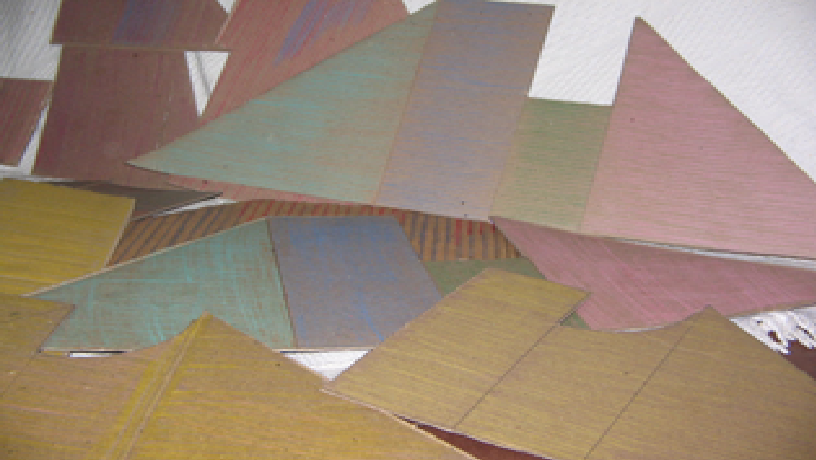
\includegraphics[width=0.9\linewidth]{Figuras/OI.png}\\
\vspace{2mm}
\end{figure}

Numere figuras e tabelas em sequencia usando algarismos arábicos (exemplo: Figura~1, Figura~2, Tabela~1, Tabela 2). Faça referência a elas no texto como "Tabela~\ref{tab:coeficiente}" e "Figura~\ref{fig:pecas}".

Denomine os eixos coordenados em gráficos, incluindo as respectivas unidades, sempre que aplicável. Da mesma forma, denomine colunas/linhas em tabelas, com respectivas unidades, caso aplicável.

\subsection{Citações}
Identifique no texto, após o trecho citado, as referências entre parênteses no seguinte padrão: sobrenome do autor em letras maiúsculas e o ano, conforme a norma da ABNT. Exemplos: um autor:  \cite{TOZZI2004}; dois autores: \cite{JOAO2000} ; três ou mais autores: \cite{PEDRO2100}. Caso ultrapasse cinco linhas, a citação deverá ser apresentada em itálico e com recuo. Outros exemplos de citações \cite{Jaffe79} \cite{Ieee2000}.

\subsection{Autorizações/Reconhecimento}
Os autores são responsáveis por garantir o direito de publicar todo o conteúdo de seu trabalho. Se material com direitos autorais foi usado na preparação do mesmo, pode ser necessário obter a devida autorização do detentor dos direitos para a publicação do material em questão.

\section{CONSIDERAÇÕES FINAIS}
O trabalho deverá ser feito com editor Word for Windows e enviado eletronicamente através do JEMS, no formato PDF, seguindo-se orientações contidas na página do evento. Não serão aceitos trabalhos enviados por correio, por fax ou por e-mail. Será acusado, via sistema do evento, o recebimento e a aceitação ou não de cada um dos trabalhos enviados.


Os autores devem combinar com os coautores quem realizará a submissão do trabalho no sistema JEMS. Trabalhos enviados em duplicata serão desabilitados pelo Comitê Técnico Científico para participar do COBENGE 2017.

\subsection{\it \textbf {Agradecimentos}}
Nesta seção poderão ser incluídos reconhecimentos de apoios recebidos de pessoas físicas e instituições. Esta seção deve estar localizada entre o fim do corpo do texto e a lista de referências. Digite somente “Agradecimentos” em negrito e itálico, com alinhamento à esquerda e digite o texto na linha seguinte.


\renewcommand{\refname}{REFERÊNCIAS BIBLIOGRÁFICAS}
\bibliography{cobengebib}

INSTRUCTIONS FOR PREPARATION AND SUBMISSION OF WORKS TO THE SCIENTIFIC COMMITTEE OF XLIV BRAZILIAN CONGRESS OF ENGINEERING EDUCATION

\begin{abstract}
This document presents detailed instructions...
\end{abstract}
%
\begin{keywords}
first one, second word …
\end{keywords}

\end{document}



